\chapter{Grundlagen}

Die Positionsbestimmung besteht aus drei elementaren Teilen. Der Kamerakalibrierung, welche das Bild entzerrt und wichtige Parameter der Kamera zurückliefert, welche für die Bestimmung der Perspektive wichtig sind. Anhand dieser Daten wird mittels der von OpenCV bereitgestellten Funktion die Perspektive von der Kamera zur Projektionsfläche bestimmt. Zuletzt wird mit Hilfe von Rodrigues die Rotation der Projektionsfläche angepasst. Diese drei Teile wollen wir hier nun etwas detaillierter erklären.

\section{Kamerakalibrierung}
Unsere Motivation einen Kalibrierungsprozess in die Applikation einzubauen war zum einen um zu verifizieren, ob unsere eingesetzten Kameras, wie von uns angenommen, verzerrungsfrei arbeiten. Zum anderen benötigen wir die intrinsischen Parameter der Kamera um ein Objekt korrekt in eine Augmented Reality Szene projizieren zu können. Die extrinsischen Parameter sind in unserem Fall zweitrangig, da diese von der Position der Kamera zur Projektionsfläche abhängen und somit zur Laufzeit stetig neu berechnet werden müssen.
\paragraph{}
Die Kalibrierung an sich umfasst die Analyse einer Serie von Projektionen von charakteristischen Punkten eines Musters, wobei die Position dieser "Feature Points" mit hoher Präzision bekannt ist. Die Position und die Distanz zwischen den einzelnen Punkten innerhalb der Projektion liefern Rückschlüsse bezüglich der Verzerrung innerhalb von dieser als auch Informationen bezüglich der intrinsischen und extrinsischen Eigenschaften des Aufnahmegerätes. 
\paragraph{}
Das Muster welches in diesem Projekt verwendet wurde ist ein Schachbrett. Durch die hohen Kontraste eines Schachbrettes lassen sich die Schnittpunkte der einzelnen Kacheln mit einer sehr hohen Präzision ermitteln. Die Projektionen sind in unserem Fall Aufnahmen des Schachbrettes aus verschiedenen Blickrichtungen. Wir haben uns für diese Basis für den Kalibrierungsprozess entschieden, weil diese sich in diversen Projekten bewährt hat und weil OpenCV bereits entsprechende Funktionen enthält um mit dieser Datengrundlage die Kalibrierung zu vollziehen. 

\section{Intrinsische Parameter}
Die intrinsischen Parameter einer Kamera bestehen aus zwei Komponenten: der Brennweite $f_x$ und $f_y$ und der Abweichung des Zentrum des Sensors zur optischen Bildmitte $c_x$ und $c_y$. Was diese zwei Eigenschaften beschreiben ist die interne Geometrie der Kamera, d.h. wie die aufgenommene Szene in ein 2D-Bild abgebildet wird. Somit ist klar, warum diese Parameter für die Ermittlung der Perspektive so wichtig sind. Zu beachten ist, dass die ermittelte Brennweite $f$ nicht die physische Brennweite sondern eine Kombination $Fs$ ist. $F$ gibt die Brennweite in mm an und $s$ die Skalierung von Pixel pro mm auf dem Sensor. Somit kann mittels $f$ die Pixelinformation bestimmt werden. Das Resultat ist eine einfache Abbildung eines Weltpunktes $(X, Y, Z)$ auf einen Bildpunkt $(x_i, y_i)$ welche wie folgt beschrieben ist.

\begin{equation}
x_i = f_x (\frac{X}{Z}) + c_x,   y_i = f_y (\frac{Y}{Z}) + c_y
\end{equation}
\noindent
Diese zwei Operationen können nun auch in eine homogene Operation zusammengefasst werden.

\begin{equation}
\begin{bmatrix}
x \\ y \\ w
\end{bmatrix} 
=
\begin{bmatrix}
f_x & 0 & c_x \\
0 & f_y & c_y \\
0 & 0 & 1
\end{bmatrix} 
\begin{bmatrix}
X \\ Y \\ Z
\end{bmatrix} 
\end{equation}
\noindent
Da die intrinsischen Parametereigenschaften der Hardware und unabhängig von der Umgebung sind, müssen sie für jedes Aufnahmegerät nur einmal zu Begin bestimmt werden und können anschliessend fix in der Applikation hinterlegt werden.

\section{Verzerrung}
Es gibt zwei Arten von Verzerrungen welche bei Aufnahmen mit Kameras entstehen können: radiale und tangentiale. Radiale Verzerrungen sind auf die gewölbte Form der Linsen zurückzuführen. Im Zentrum des Bildes ist die radiale Verzerrung noch bei null und nimmt gegen den Rand immer wie stärker zu. Theoretisch währe es möglich eine nahezu perfekte parabolische Linse herzustellen, jedoch wäre diese viel zu kostspielig in der Produktion. Deshalb werden allgemein sphärische Linsen eingesetzt.

\begin{figure}[!ht]
\centering
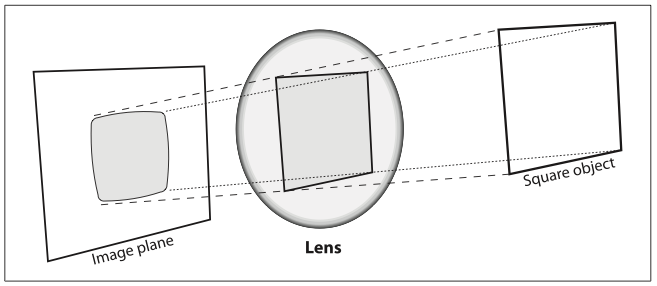
\includegraphics[scale=0.5]{images/radial-disortion.png} 
\caption{Strahlen welche die Linse weiter weg vom Zentrum passieren werden stärker abgelenkt als solche nahe dem Zentrum. Darum erschein die Projektion verzerrt.\protect\cite{learningopencv}}
\label{fig:radial-disortion}
\end{figure}
\noindent
Tangentiale Verzerrungen werden durch Ungenauigkeiten bei der Zusammensetzung des optischen Systems verursacht. Diese entstehen, wenn die Linse nicht komplett parallel zum Sensor steht.

\begin{figure}[!ht]
\centering
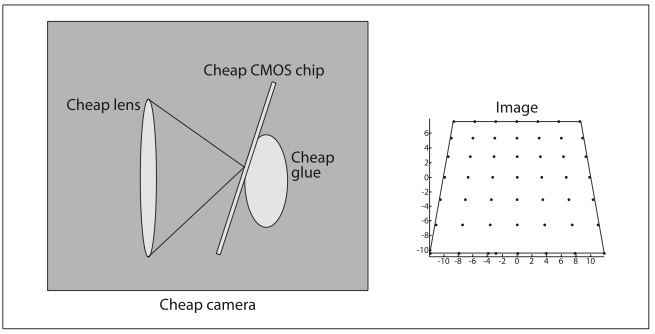
\includegraphics[scale=0.5]{images/tangential-disortion.png} 
\caption{Tangentiale Verzerrung aufgrund von Fehlern im optischen System.\protect\cite{learningopencv}}
\label{fig:tangential-disortion}
\end{figure}

\section{Koordinatensysteme}
Um den Kalibrierungsprozess zu verstehen, muss man auch die einzelnen Koordinatensysteme kennen, welche bei der Aufnahme eines Bildes durchlaufen werden. Deshalb möchten wir diese Hier kurz erläutern.

\paragraph{Weltkoordinatensystem} Dieses ist das Koordinatensystem in welchen die "reale Welt" gemessen wird und ist dreidimensional. Dies ist der Ursprung der Bilddaten.

\paragraph{Standardkoordinatensystem} Dieses dreidimensionale Koordinatensystem hat den Ursprung im Projektionszentrum. Seine Z-Achse verläuft entlang der optischen Achse.

\paragraph{Bildkoordinatensystem} Dieses hat seinen Ursprung beim Schnittpunkt der optischen Achse und der Bildebene. Die x- und y-Achse sind parallel zur X- bzw. Y-Achse des Standardkoordinatensystems.

\paragraph{Pixelkoordinatensystem} Das Pixelkoordinatensystem hat seinen Ursprung beim Korrigierten Punkt $c_x$ \/ $c_y$  und seine x- und y-Achse sind parallel zur x- bzw. y-Achse des Bildkoordinatensystem.

\paragraph{} Während dem Abbildungsprozess durchlaufen die einzelnen Bildimformationen nun diese Systeme wie folgt: Weltkoordinaten $\Rightarrow$ Standardkoordinaten $\Rightarrow$ Bildkoordinaten $\Rightarrow$ Pixelkoordinaten

\section{Implementierung}
Die Funktionalität für die Kalibrierung ist in der Klasse CameraCalibration implementiert. Da alle benötigten Algorithmen bereits in OpenCV implementiert sind, ist der Kalibrierungsprozess relativ einfach umzusetzen. OpenCV selbst verwendet das Verfahren, welches 1998 von Zhang\cite{zhang} entwickelt wurde. Dabei werden die einzelnen Parameter nicht exakt berechnet sondern mittels einer "Maximum likelihood estimation" mit einer hohen Präzision geschätzt. Eine präzise Schätzung erfordert jedoch eine breite Datenbasis. Deshalb reicht es nicht aus, nur eine Aufnahme des Schachbrettmusters als Input zu liefern. Empfohlen werden 15 - 20 Aufnahmen aus möglichst verschiedenen Blickwinkeln. Da die Erkennung des Musters nicht 100\% treffgenau ist, haben wir uns dazu entschieden immer min. 20 Aufnahmen zu verwenden. So können wir davon ausgehen, dass immer mehr als 15 erfolgreiche Erkennungen stattfinden.

\paragraph{}
Die Funktion \textit{CameraCalibration::cornerSubPix} akzeptiert eine Liste von aufnahmen des Schachbrettmusters. Als zweiter Parameter muss die Grösse des Brettes angegeben werden (die Anzahl innerer Eckpunkte in horizontaler und vertikaler Richtung). Dabei sollten die Breite ungerade und die Höhe gerade sein und das Muster sollte breiter als hoch sein. Wir haben uns für ein 6x9 grosses Muster entschieden, da dies die geläufigste Grösse zu sein scheint. Nun wird mittels \textit{CameraCalibration::findChessboardPoints} die Erkennung durchgeführt. Dabei müssen die \textit{objectCorners} (Bildkoordinatensystem) auf einen initialen Erwartungswert gesetzt werden.

\begin{c++code}
for(int i = 0; i < boardSize.height; i++)
{
    for(int j = 0; j < boardSize.width; j++)
    {
        //110 = size of one square on the board
        objectCorners.push_back(
            cv::Point3f(i * 110, j * 110, 0.0f)
        );
    }
}
\end{c++code}
\noindent
Diese Punkte werden für die Erkennung des Schachbrettes noch nicht benötigt sondern erst bei der Kalibrierung. Anschliessend wird die OpenCV eigene Funktion zur Ermittlung des Musters aufgerufen.

\begin{c++code}
cv::findChessboardCorners(
    image, 
    boardSize, 
    imageCorners, 
    CV_CALIB_CB_ADAPTIVE_THRESH | CV_CALIB_CB_FILTER_QUADS
);
\end{c++code}
\noindent
Da \textit{cv::findChessboardCorners} nur die ungefähre Position der Eckpunkte ermittelt, müssen die ermittelten Daten mit Hilfe von \textit{cv::cornerSubPix} verfeinert werden. Würde man dies nicht tun, so würde es zu Fehlern bei der Kalibrierung führen. Das genaue Vorgehen der Funktion kann der OpenCV Dokumentation \footnote{\protect\url{http://opencv.willowgarage.com/documentation/cpp/imgproc_feature_detection.html#cv-cornersubpix}} entnommen werden.

\paragraph{}War die Erkennung des Schachbrettes erfolgreich, so entspricht die Anzahl an gefundenen \textit{imageCorners} der zuvor definierten Brettgrösse von 9x6, sprich 54. Alle erfolgreichen Versuche werden anschliessend in einer Liste abgelegt. Was zu beachten ist, und was uns einiges an Zeit gekostet hat, ist, dass die \textit{imageCorners} und die \textit{objectCorners} die gleiche Dimension haben müssen. Ist dies nicht der Fall, so schlägt die Kalibrierung mit einer kryptischen Meldung fehl.

\paragraph{} Nun kann mittels \textit{CameraCalibration::calibrate} die Kalibrierung vorgenommen werden. Diese ist die Voraussetzung für die anschliessende Entzerrung des Bildes welche in \textit{CameraCalibration::remap} stattfindet. Nach jeder Kalibrierung müssen die Daten für die Entzerrung initialisiert werden. Hier ist auch der Punkt, wo wir die Kameramatrix erhalten, welche die intrinsischen Parameter enthält.

\section{Auswertung} Das nun entzerrte Bild kann mit dem Ursprungsbild verglichen werden um zu eruieren ob das optische System Verzerrungen verursacht (Abb. \ref{fig:chessboard-disorted} und \ref{fig:chessboard-undisorted}). Bei den von uns getesteten Kameras konnten wir keine Verzerrungen feststellen. Dabei würden zwei Smartphone-Kameras (iPhone 4 und HTC Desire Z) und zwei Webcams (iSight Kamera eines MacBook Pro und die integrierte Kamera eines HP Notebooks) getestet. Hier stellt sich aber die Frage, ob die getesteten optischen Systeme so kompakt sind, dass die Verzerrungen optisch nicht erfasst werden können oder ob auf Hardwareebene bereits eine Korrektur stattfindet und die API nur Zugriff auf dieses Bild hat. Hierzu konnten wir Seitens der Hardwarehersteller keine Informationen finden. Abb. \ref{fig:calibration} zeigt ein Beispiel einer Kamera welche verzerrte Bilder zurückgibt.

\begin{figure}[!ht]
\centering
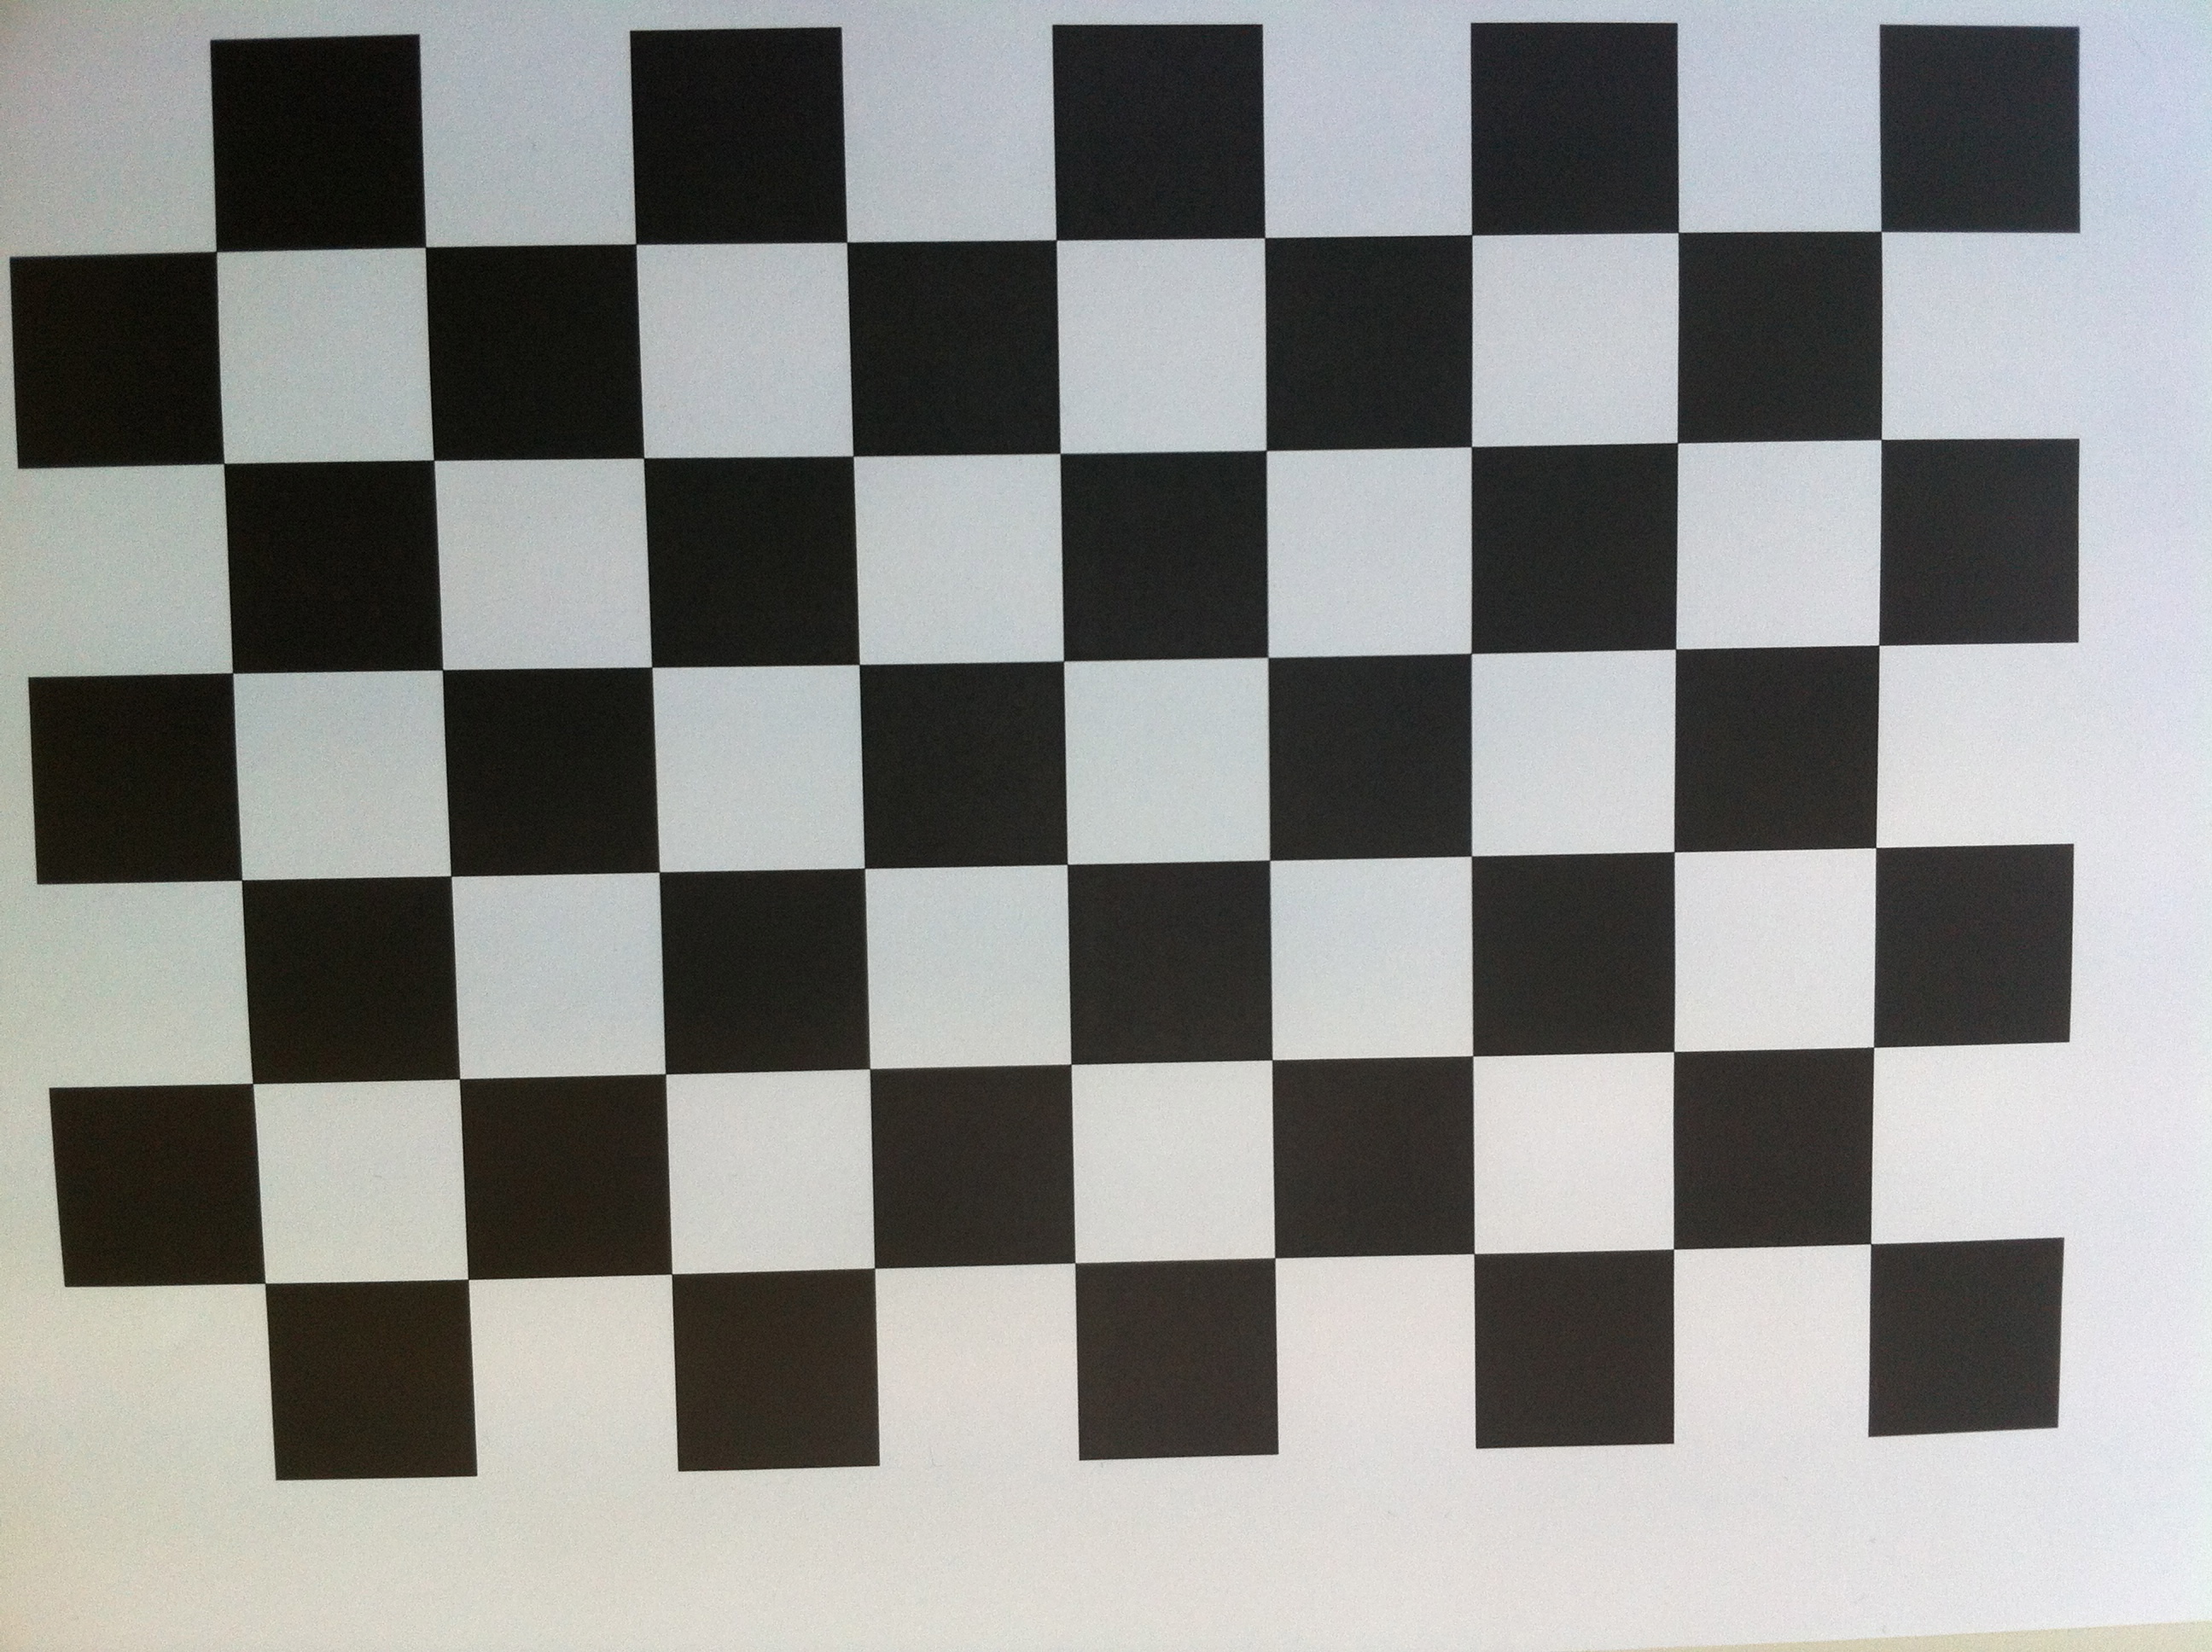
\includegraphics[scale=0.1]{images/chessboard-disorted.jpg} 
\caption{Originalbild}
\label{fig:calib-d}
\end{figure}

\begin{figure}[!ht]
\centering
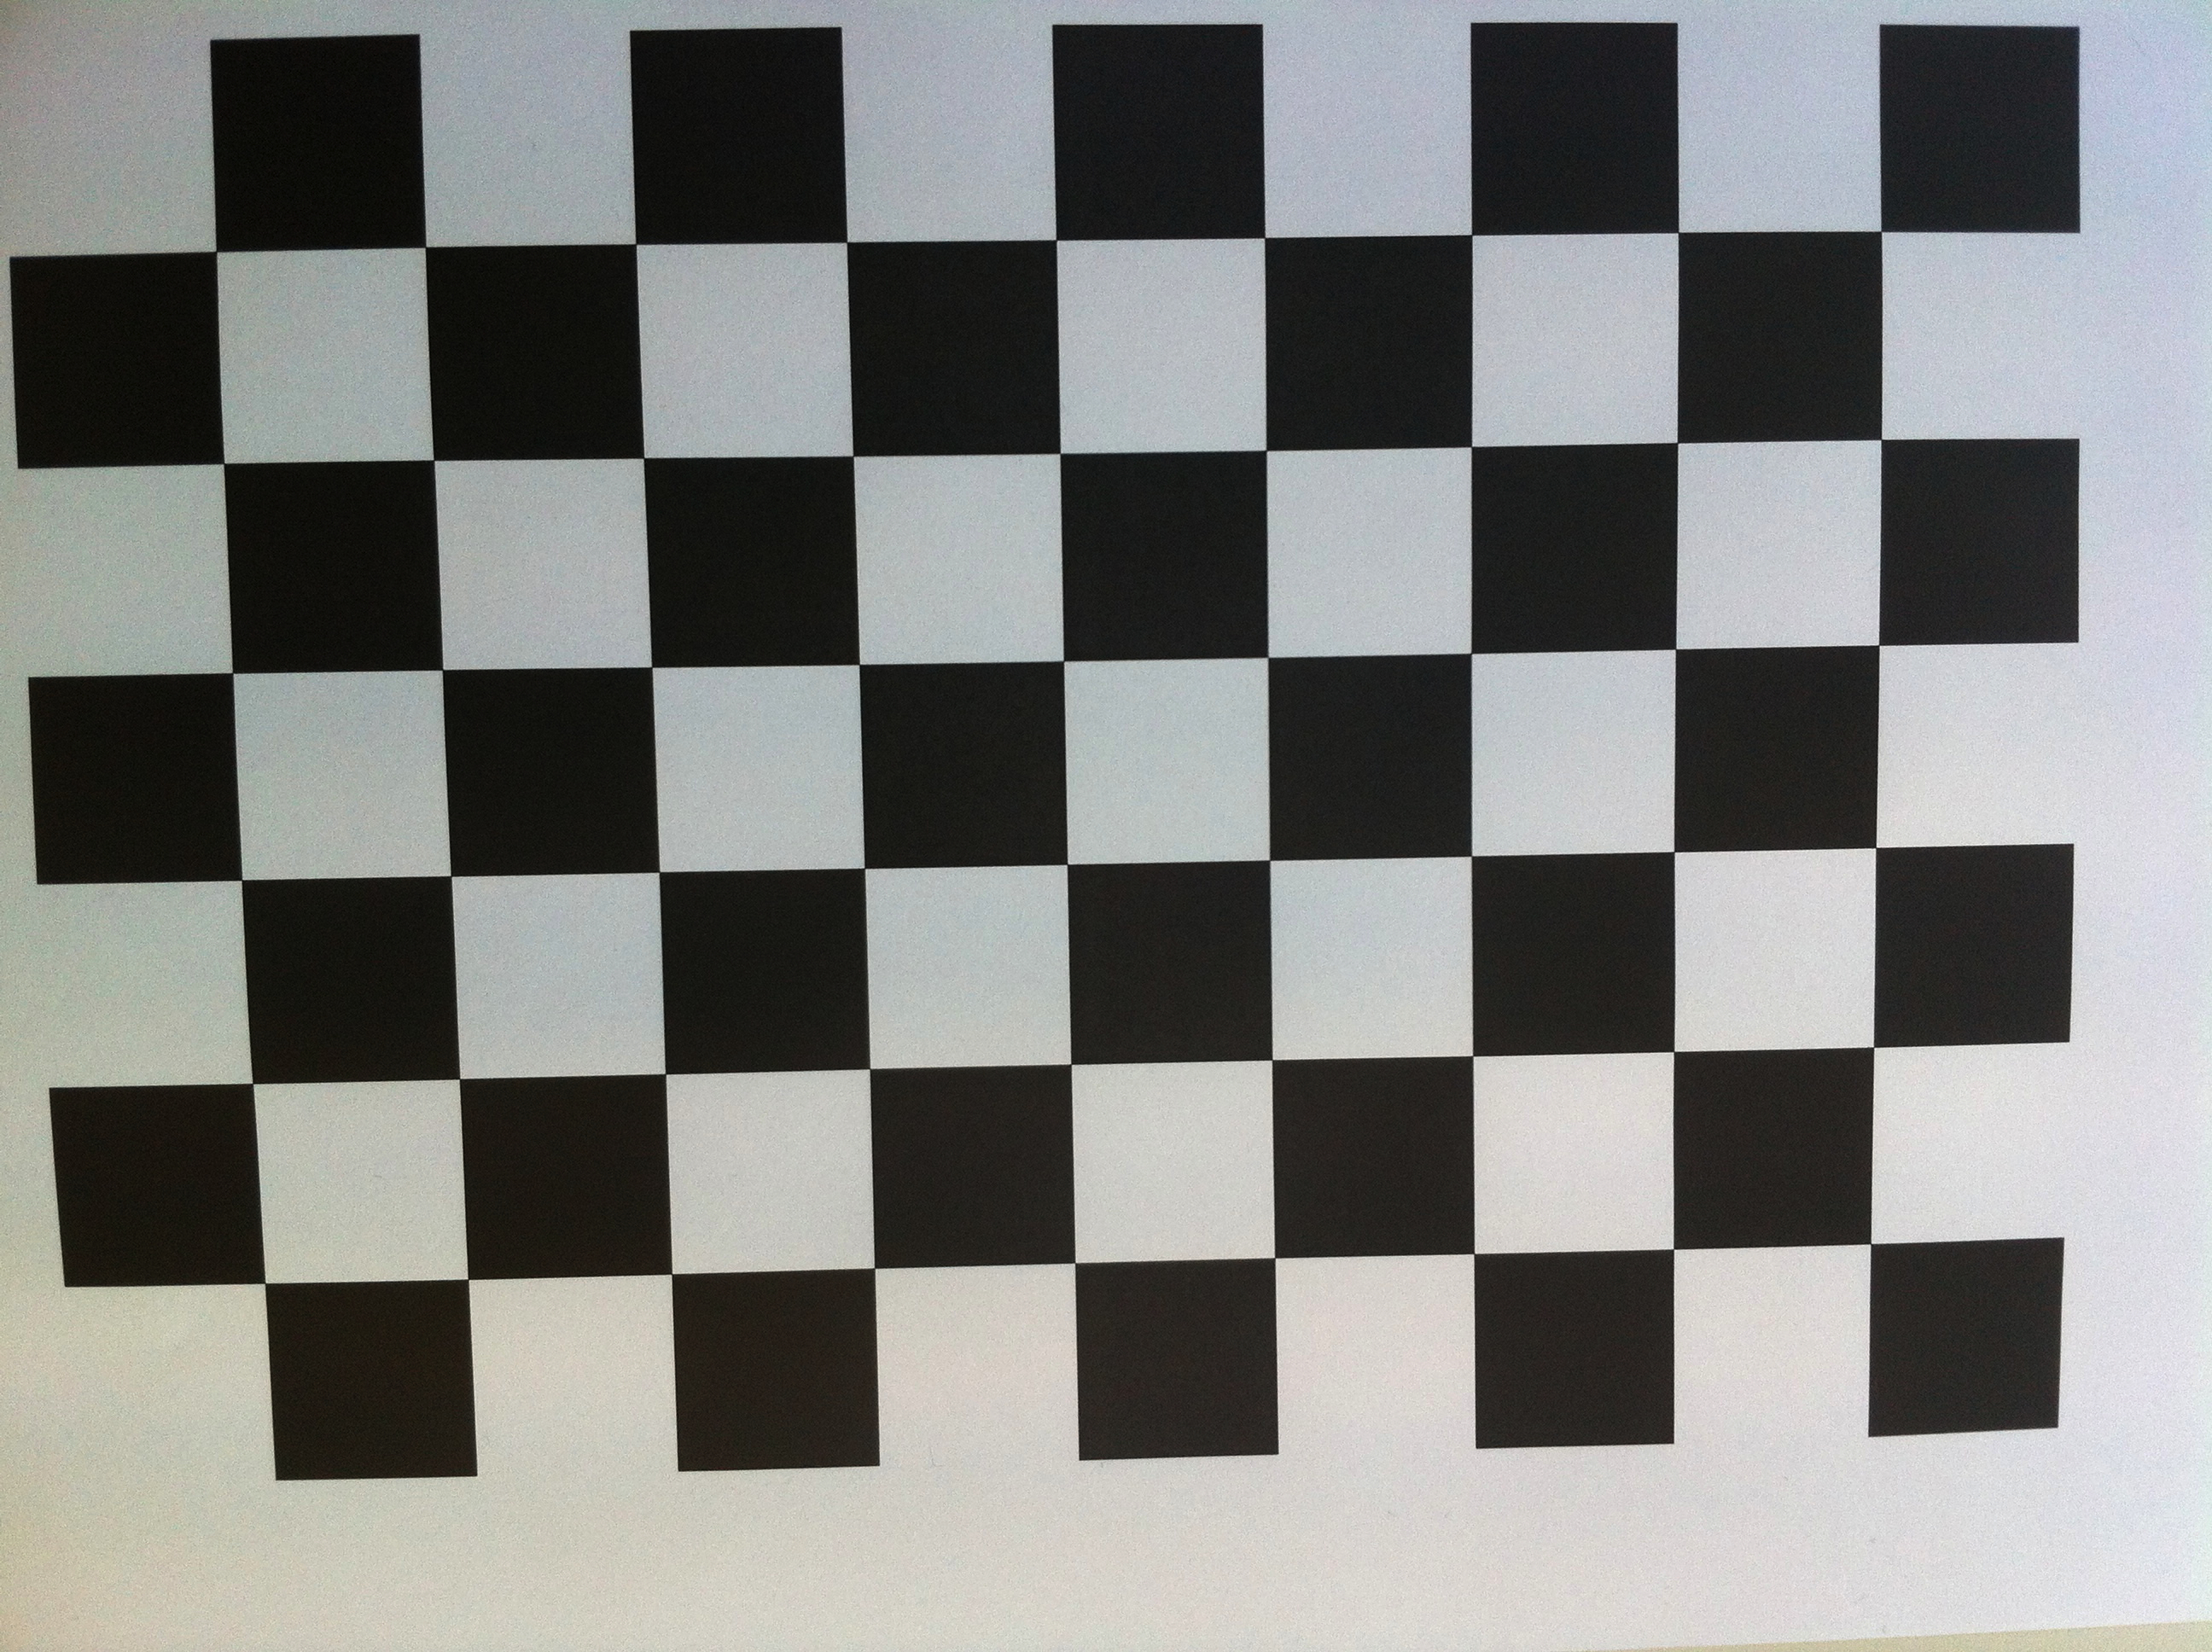
\includegraphics[scale=0.1]{images/chessboard-undisorted.jpg} 
\caption{Entzertes Bild}
\label{fig:chessboard-undisorted}
\end{figure}

\begin{figure}[!ht]
\centering
\subfloat[Ausgangsbild]{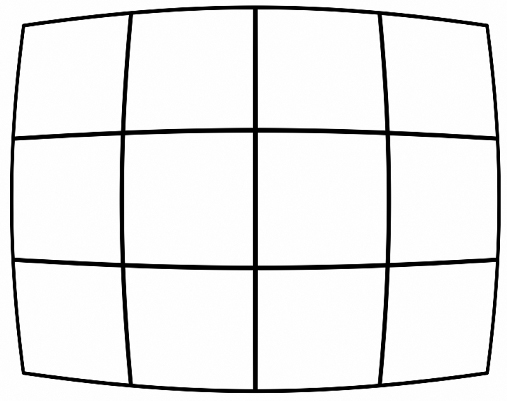
\includegraphics[width=0.49\textwidth]{images/calib-distorted.jpg}}
\subfloat[Korrigiertes Bils]{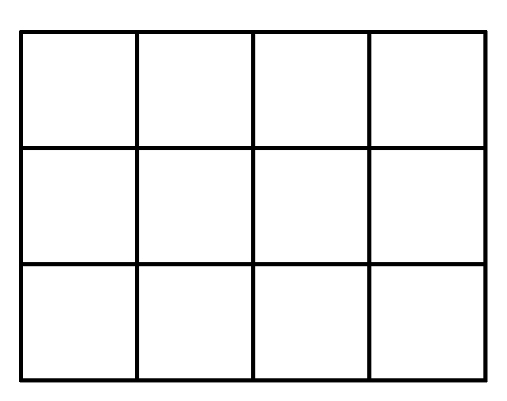
\includegraphics[width=0.49\textwidth]{images/calib-undistorted.jpg}}
\caption{Zum vergleich ein Bild mit einer Kamera welche Verzerrungen verursacht (a) und die entzerrte Variante (b)}
\label{fig:calibration}
\end{figure}

\section{Projektionsmodell}
\label{sec:projektionsmodell}

Alle Funktionen in OpenCV arbeiten nach dem sogenannten Pinhole Camera Modell. Dabei werden die 3D-Punkte einer Szene mittels perspektivischer Transformation auf die Bildebene projiziert.

\begin{equation}
\vec{p^p} = K [R|t] \vec{p^i}
\end{equation}
\noindent
Die ausgeschriebene Form zum besseren Verständnis:

\begin{equation}
\begin{bmatrix}	
p^c_x \\ p^c_y \\ 1
\end{bmatrix} 
=
\begin{bmatrix}
f_x & 0 & c_x \\
0 & f_y & c_y \\
0 & 0 & 1
\end{bmatrix} 
\begin{bmatrix}
r_{11} & r_{12} & r_{13} & t_1 \\
r_{21} & r_{22} & r_{23} & t_2 \\
r_{31} & r_{32} & r_{33} & t_3
\end{bmatrix} 
\begin{bmatrix}
p^i_x \\ p^i_y \\ p^i_z \\ 1
\end{bmatrix} 
\end{equation}
\noindent
Ein Punkt $(p^i_x, p^i_y, p^i_z)$ im dreidimensionalen Raum wird dadurch auf einen zweidimensionalen Punkt in der Bildebene projiziert. Die Kamera-Matrix $K$ enthält dabei die intrinsischen Parameter und welche nur einmal zu Begin berechnet werden müssen. Die kombinierte Rotations- und Translationsmatrix $[R|t]$ überführt Objekt- in Kamera-Koordinaten, also in die Position, aus der das Objekt von der Kamera gesehen wird. Diese Matrix stellt die extrinsischen Parameter dar und muss anhand einer \textit{Pose Estimation} berechnet werden.

\section{Pose Estimation}
Bei der 3D Pose Estimation wird die Position sowie die Rotation eines Objekts in einem zweidimensionalen Bildes berechnet. Dadurch erhält man die Position des 3D-Objekts im dreidimensionalen Objektraum. Es gibt eine vielzahl an Algorithmen die sich diesem Problem widmen.

\paragraph{}
Zusätzliche Details zu diesem Thema folgen in Kapitel \ref{chap:projektion}.


\section{Rotation}
Eine 3x3 Matrix ist die geläufigste Methode wenn es darum geht eine Rotation im Raum zu vollziehen. Multipliziert man den Vektor mit der Matrix welche die entsprechenden Parameter enthält, so erhält man als Resultat den rotierten Vektor. Der Nachteil dabei ist, dass man für die Rotation jeder Achse andere Parameter der Matrix anpassen muss. Man kann die drei Matrizen zu einer zusammenfassen, jedoch wird die Prozedur dadurch noch unübersichtlicher. Da die Rotationsmatrizen nur drei Freiheitsgrade haben, ist der Gedanke nahe, die Informationen in einen Vektor abzubilden. Und genau hier setzt die in OpenCV implementierte Rodrigues-Transformation an. Nicht nur für uns Menschen ist ein Vektor einfacher lesbar, auch für numerische Optimierungen ist es einfacher mit einem Drei-Komponenten-Vektor zu arbeiten als mit einer 3x3 Matrix.

\paragraph{}
Rodrigues nutzt die Richtung des Vektors um die Rotationsachse und die Länge des Vektors um den Winkel der Rotation – im Gegenuhrzeigersinn – abzubilden. Sei $r$ ein dreidimensionaler Vektor 

\begin{equation}
\begin{pmatrix} r_x \\ r_y \\ r_z \end{pmatrix}
\end{equation}
\noindent
Dieser Vektor bildet implizit den Winkel anhand seiner Länge ab.

\begin{equation}
\theta = \sqrt{{r_x}^2 + {r_y}^2 + {r_z}^2}
\end{equation}
\noindent
Anhand dieser Repräsentation kann die Rotationsmatrix wie folgt wieder hergestellt werden:

\begin{equation}
R = \cos(\theta) * I + (1 - \cos(\theta)) * r * r^T + \sin(\theta) * 
\begin{bmatrix}
0 & -r_z & r_y \\
r_z & 0 & -r_x \\
r_y & r_x & 0
\end{bmatrix}
\end{equation}
\noindent
Umgekehrt kann man aus der Rotationsmatrix die Rodrigues-Darstellung wie folgt ableiten:

\begin{equation}
\sin(\theta) * 
\begin{bmatrix}
0 & -r_z & r_y \\
r_z & 0 & -r_x \\
r_y & r_x & 0
\end{bmatrix}
= 
\frac{R - R^T}{2}
\end{equation}
\noindent
Und genau diese zwei Möglichkeiten sind in \textit{cv::Rodrigues} implementiert. Wird als erster Parameter ein 3D-Vektor und als zweiter eine 3x3 Matrix übergeben so wird der Vektor zu einer Matrix transformiert. Will man die Operation umkehren, so müssen nur die Parameter-Typen in umgekehrter Reihenfolge übergeben werden.
